% Created by tikzDevice version 0.12.5 on 2023-11-24 23:42:35
% !TEX encoding = UTF-8 Unicode
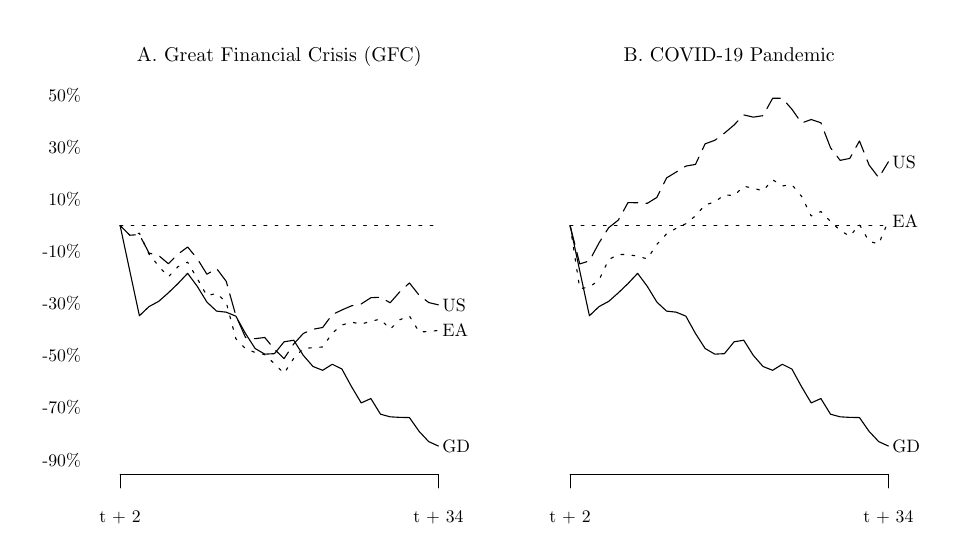
\begin{tikzpicture}[x=1pt,y=1pt]
\definecolor{fillColor}{RGB}{255,255,255}
\path[use as bounding box,fill=fillColor,fill opacity=0.00] (0,0) rectangle (325.21,180.67);
\begin{scope}
\path[clip] ( 28.80, 19.20) rectangle (153.01,161.47);
\definecolor{drawColor}{RGB}{0,0,0}

\path[draw=drawColor,line width= 0.4pt,line join=round,line cap=round] ( 33.40,109.16) --
	( 36.89, 92.80) --
	( 40.37, 76.57) --
	( 43.86, 79.89) --
	( 47.34, 81.77) --
	( 50.83, 84.85) --
	( 54.31, 88.20) --
	( 57.80, 91.91) --
	( 61.28, 87.20) --
	( 64.77, 81.50) --
	( 68.25, 78.25) --
	( 71.74, 77.87) --
	( 75.22, 76.43) --
	( 78.71, 70.16) --
	( 82.19, 64.73) --
	( 85.68, 62.70) --
	( 89.16, 62.87) --
	( 92.65, 67.15) --
	( 96.13, 67.74) --
	( 99.62, 62.23) --
	(103.10, 58.24) --
	(106.59, 56.86) --
	(110.07, 59.04) --
	(113.56, 57.30) --
	(117.04, 50.91) --
	(120.53, 45.07) --
	(124.01, 46.66) --
	(127.50, 41.00) --
	(130.98, 40.05) --
	(134.47, 39.85) --
	(137.95, 39.78) --
	(141.44, 34.80) --
	(144.92, 31.08) --
	(148.41, 29.50);
\end{scope}
\begin{scope}
\path[clip] ( 28.80, 19.20) rectangle (153.01,161.47);
\definecolor{drawColor}{RGB}{0,0,0}

\path[draw=drawColor,line width= 0.4pt,dash pattern=on 1pt off 3pt ,line join=round,line cap=round] ( 33.40,109.16) --
	(148.41,109.16);
\end{scope}
\begin{scope}
\path[clip] (  0.00,  0.00) rectangle (325.21,180.67);
\definecolor{drawColor}{RGB}{0,0,0}

\path[draw=drawColor,line width= 0.4pt,line join=round,line cap=round] ( 33.40, 19.20) -- (148.41, 19.20);

\path[draw=drawColor,line width= 0.4pt,line join=round,line cap=round] ( 33.40, 19.20) -- ( 33.40, 14.40);

\path[draw=drawColor,line width= 0.4pt,line join=round,line cap=round] (148.41, 19.20) -- (148.41, 14.40);

\node[text=drawColor,anchor=base,inner sep=0pt, outer sep=0pt, scale=  0.64] at ( 33.40,  1.92) {t + 2};

\node[text=drawColor,anchor=base,inner sep=0pt, outer sep=0pt, scale=  0.64] at (148.41,  1.92) {t + 34};

\node[text=drawColor,anchor=base east,inner sep=0pt, outer sep=0pt, scale=  0.64] at ( 19.20, 22.27) {-90\%};

\node[text=drawColor,anchor=base east,inner sep=0pt, outer sep=0pt, scale=  0.64] at ( 19.20, 41.08) {-70\%};

\node[text=drawColor,anchor=base east,inner sep=0pt, outer sep=0pt, scale=  0.64] at ( 19.20, 59.90) {-50\%};

\node[text=drawColor,anchor=base east,inner sep=0pt, outer sep=0pt, scale=  0.64] at ( 19.20, 78.72) {-30\%};

\node[text=drawColor,anchor=base east,inner sep=0pt, outer sep=0pt, scale=  0.64] at ( 19.20, 97.54) {-10\%};

\node[text=drawColor,anchor=base east,inner sep=0pt, outer sep=0pt, scale=  0.64] at ( 19.20,116.36) {10\%};

\node[text=drawColor,anchor=base east,inner sep=0pt, outer sep=0pt, scale=  0.64] at ( 19.20,135.18) {30\%};

\node[text=drawColor,anchor=base east,inner sep=0pt, outer sep=0pt, scale=  0.64] at ( 19.20,154.00) {50\%};

\node[text=drawColor,anchor=base west,inner sep=0pt, outer sep=0pt, scale=  0.65] at (149.84, 27.27) {GD};
\end{scope}
\begin{scope}
\path[clip] ( 28.80, 19.20) rectangle (153.01,161.47);
\definecolor{drawColor}{RGB}{0,0,0}

\path[draw=drawColor,line width= 0.4pt,dash pattern=on 7pt off 3pt ,line join=round,line cap=round] ( 33.40,109.16) --
	( 36.89,105.67) --
	( 40.37,105.89) --
	( 43.86, 99.22) --
	( 47.34, 98.33) --
	( 50.83, 95.38) --
	( 54.31, 98.82) --
	( 57.80,101.41) --
	( 61.28, 97.20) --
	( 64.77, 91.57) --
	( 68.25, 93.65) --
	( 71.74, 89.02) --
	( 75.22, 76.66) --
	( 78.71, 68.73) --
	( 82.19, 68.30) --
	( 85.68, 68.72) --
	( 89.16, 64.46) --
	( 92.65, 61.09) --
	( 96.13, 66.38) --
	( 99.62, 70.19) --
	(103.10, 71.69) --
	(106.59, 72.33) --
	(110.07, 77.00) --
	(113.56, 78.66) --
	(117.04, 80.17) --
	(120.53, 80.84) --
	(124.01, 83.09) --
	(127.50, 83.26) --
	(130.98, 81.26) --
	(134.47, 85.23) --
	(137.95, 88.43) --
	(141.44, 84.00) --
	(144.92, 81.35) --
	(148.41, 80.50);
\end{scope}
\begin{scope}
\path[clip] (  0.00,  0.00) rectangle (325.21,180.67);
\definecolor{drawColor}{RGB}{0,0,0}

\node[text=drawColor,anchor=base west,inner sep=0pt, outer sep=0pt, scale=  0.65] at (149.84, 78.27) {US};
\end{scope}
\begin{scope}
\path[clip] ( 28.80, 19.20) rectangle (153.01,161.47);
\definecolor{drawColor}{RGB}{0,0,0}

\path[draw=drawColor,line width= 0.4pt,dash pattern=on 1pt off 3pt ,line join=round,line cap=round] ( 33.40,109.16) --
	( 36.89,105.70) --
	( 40.37,106.38) --
	( 43.86, 98.82) --
	( 47.34, 94.51) --
	( 50.83, 90.61) --
	( 54.31, 94.29) --
	( 57.80, 95.95) --
	( 61.28, 90.01) --
	( 64.77, 83.78) --
	( 68.25, 84.70) --
	( 71.74, 81.45) --
	( 75.22, 68.28) --
	( 78.71, 64.64) --
	( 82.19, 63.31) --
	( 85.68, 62.54) --
	( 89.16, 59.21) --
	( 92.65, 55.74) --
	( 96.13, 61.17) --
	( 99.62, 64.80) --
	(103.10, 65.01) --
	(106.59, 65.30) --
	(110.07, 70.30) --
	(113.56, 73.22) --
	(117.04, 74.27) --
	(120.53, 73.54) --
	(124.01, 74.60) --
	(127.50, 75.34) --
	(130.98, 71.69) --
	(134.47, 75.13) --
	(137.95, 76.50) --
	(141.44, 70.74) --
	(144.92, 70.85) --
	(148.41, 71.27);
\end{scope}
\begin{scope}
\path[clip] (  0.00,  0.00) rectangle (325.21,180.67);
\definecolor{drawColor}{RGB}{0,0,0}

\node[text=drawColor,anchor=base west,inner sep=0pt, outer sep=0pt, scale=  0.65] at (149.84, 69.04) {EA};
\end{scope}
\begin{scope}
\path[clip] (  0.00,  0.00) rectangle (162.61,180.67);
\definecolor{drawColor}{RGB}{0,0,0}

\node[text=drawColor,anchor=base,inner sep=0pt, outer sep=0pt, scale=  0.72] at ( 90.90,168.60) {A. Great Financial Crisis (GFC)};
\end{scope}
\begin{scope}
\path[clip] (191.41, 19.20) rectangle (315.62,161.47);
\definecolor{drawColor}{RGB}{0,0,0}

\path[draw=drawColor,line width= 0.4pt,line join=round,line cap=round] (196.01,109.16) --
	(199.49, 92.80) --
	(202.98, 76.57) --
	(206.46, 79.89) --
	(209.95, 81.77) --
	(213.43, 84.85) --
	(216.92, 88.20) --
	(220.40, 91.91) --
	(223.89, 87.20) --
	(227.37, 81.50) --
	(230.86, 78.25) --
	(234.34, 77.87) --
	(237.83, 76.43) --
	(241.31, 70.16) --
	(244.80, 64.73) --
	(248.28, 62.70) --
	(251.77, 62.87) --
	(255.25, 67.15) --
	(258.74, 67.74) --
	(262.22, 62.23) --
	(265.71, 58.24) --
	(269.19, 56.86) --
	(272.68, 59.04) --
	(276.16, 57.30) --
	(279.65, 50.91) --
	(283.13, 45.07) --
	(286.62, 46.66) --
	(290.10, 41.00) --
	(293.59, 40.05) --
	(297.07, 39.85) --
	(300.56, 39.78) --
	(304.04, 34.80) --
	(307.53, 31.08) --
	(311.01, 29.50);
\end{scope}
\begin{scope}
\path[clip] (191.41, 19.20) rectangle (315.62,161.47);
\definecolor{drawColor}{RGB}{0,0,0}

\path[draw=drawColor,line width= 0.4pt,dash pattern=on 1pt off 3pt ,line join=round,line cap=round] (196.01,109.16) --
	(311.01,109.16);
\end{scope}
\begin{scope}
\path[clip] (  0.00,  0.00) rectangle (325.21,180.67);
\definecolor{drawColor}{RGB}{0,0,0}

\path[draw=drawColor,line width= 0.4pt,line join=round,line cap=round] (196.01, 19.20) -- (311.01, 19.20);

\path[draw=drawColor,line width= 0.4pt,line join=round,line cap=round] (196.01, 19.20) -- (196.01, 14.40);

\path[draw=drawColor,line width= 0.4pt,line join=round,line cap=round] (311.01, 19.20) -- (311.01, 14.40);

\node[text=drawColor,anchor=base,inner sep=0pt, outer sep=0pt, scale=  0.64] at (196.01,  1.92) {t + 2};

\node[text=drawColor,anchor=base,inner sep=0pt, outer sep=0pt, scale=  0.64] at (311.01,  1.92) {t + 34};

\node[text=drawColor,anchor=base west,inner sep=0pt, outer sep=0pt, scale=  0.65] at (312.45, 27.27) {GD};
\end{scope}
\begin{scope}
\path[clip] (191.41, 19.20) rectangle (315.62,161.47);
\definecolor{drawColor}{RGB}{0,0,0}

\path[draw=drawColor,line width= 0.4pt,dash pattern=on 7pt off 3pt ,line join=round,line cap=round] (196.01,109.16) --
	(199.49, 95.29) --
	(202.98, 96.40) --
	(206.46,102.92) --
	(209.95,108.40) --
	(213.43,111.14) --
	(216.92,117.44) --
	(220.40,117.41) --
	(223.89,117.20) --
	(227.37,119.34) --
	(230.86,126.39) --
	(234.34,128.49) --
	(237.83,130.64) --
	(241.31,131.27) --
	(244.80,138.70) --
	(248.28,139.96) --
	(251.77,142.55) --
	(255.25,145.50) --
	(258.74,149.14) --
	(262.22,148.34) --
	(265.71,148.87) --
	(269.19,155.15) --
	(272.68,155.15) --
	(276.16,151.19) --
	(279.65,146.21) --
	(283.13,147.49) --
	(286.62,146.32) --
	(290.10,137.29) --
	(293.59,132.72) --
	(297.07,133.43) --
	(300.56,139.73) --
	(304.04,131.05) --
	(307.53,126.44) --
	(311.01,132.18);
\end{scope}
\begin{scope}
\path[clip] (  0.00,  0.00) rectangle (325.21,180.67);
\definecolor{drawColor}{RGB}{0,0,0}

\node[text=drawColor,anchor=base west,inner sep=0pt, outer sep=0pt, scale=  0.65] at (312.45,129.93) {US};
\end{scope}
\begin{scope}
\path[clip] (191.41, 19.20) rectangle (315.62,161.47);
\definecolor{drawColor}{RGB}{0,0,0}

\path[draw=drawColor,line width= 0.4pt,dash pattern=on 1pt off 3pt ,line join=round,line cap=round] (196.01,109.16) --
	(199.49, 86.36) --
	(202.98, 86.90) --
	(206.46, 89.50) --
	(209.95, 96.86) --
	(213.43, 98.73) --
	(216.92, 98.69) --
	(220.40, 98.08) --
	(223.89, 97.13) --
	(227.37,102.37) --
	(230.86,106.16) --
	(234.34,108.18) --
	(237.83,109.83) --
	(241.31,112.68) --
	(244.80,116.67) --
	(248.28,117.65) --
	(251.77,120.30) --
	(255.25,119.96) --
	(258.74,123.36) --
	(262.22,122.66) --
	(265.71,121.70) --
	(269.19,125.72) --
	(272.68,123.48) --
	(276.16,123.93) --
	(279.65,119.70) --
	(283.13,112.62) --
	(286.62,114.23) --
	(290.10,110.64) --
	(293.59,107.42) --
	(297.07,105.29) --
	(300.56,109.49) --
	(304.04,103.44) --
	(307.53,102.55) --
	(311.01,110.80);
\end{scope}
\begin{scope}
\path[clip] (  0.00,  0.00) rectangle (325.21,180.67);
\definecolor{drawColor}{RGB}{0,0,0}

\node[text=drawColor,anchor=base west,inner sep=0pt, outer sep=0pt, scale=  0.65] at (312.45,108.56) {EA};
\end{scope}
\begin{scope}
\path[clip] (162.61,  0.00) rectangle (325.21,180.67);
\definecolor{drawColor}{RGB}{0,0,0}

\node[text=drawColor,anchor=base,inner sep=0pt, outer sep=0pt, scale=  0.72] at (253.51,168.60) {B. COVID-19 Pandemic};
\end{scope}
\end{tikzpicture}
